\addcontentsline{toc}{section}{Cylinder on the Corner (0)}
\section*{Cylinder on the Corner}

\subsection*{Problem}

\begin{wrapfigure}{r}{\textwidth / 2}
    \centering
    \vspace{-.75cm}
    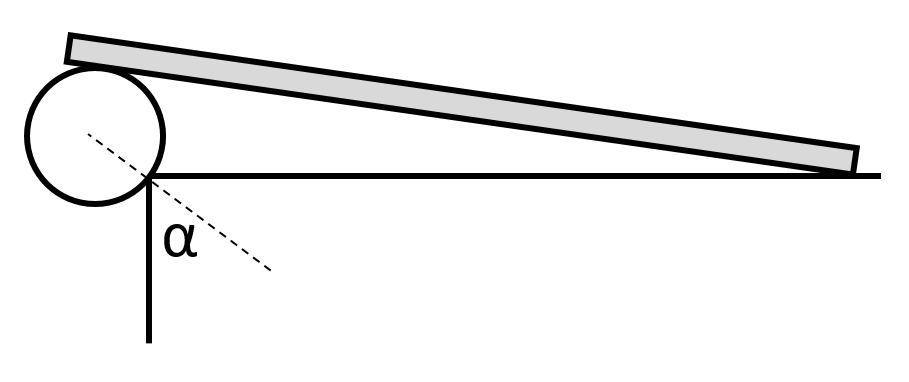
\includegraphics[width = \textwidth / 2]{P-1}
    \caption{}
    \labelf{P-1}
    \vspace{-1cm}
\end{wrapfigure}

A cylinder of mass $m$ is held on the corner of a table
by a long homogenous plank of mass $M$
in position described by $\alpha$
as shown on \reff{P-1}.
What friction coefficients must there be
between the cylinder and the table,
between the plank and the table and
between the cylinder and the plack
for this situation to be possible?
The plank is much longer than the radius of the cylinder.

\subsection*{Solution}

\begin{wrapfigure}{l}{\textwidth / 2}
    \centering

    \begin{subfigure}[l]{.5\textwidth}
        \centering
        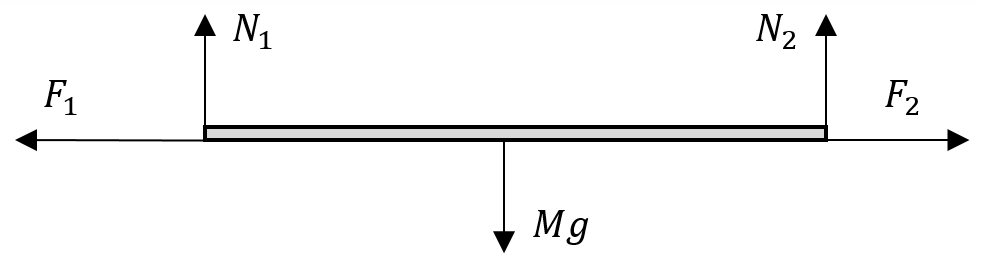
\includegraphics[width = \textwidth]{S-1}
        \caption{Forces on the plank.}
        \labelf{S-1}
    \end{subfigure}
    \hfill
    \begin{subfigure}[l]{.5\textwidth}
        \centering
        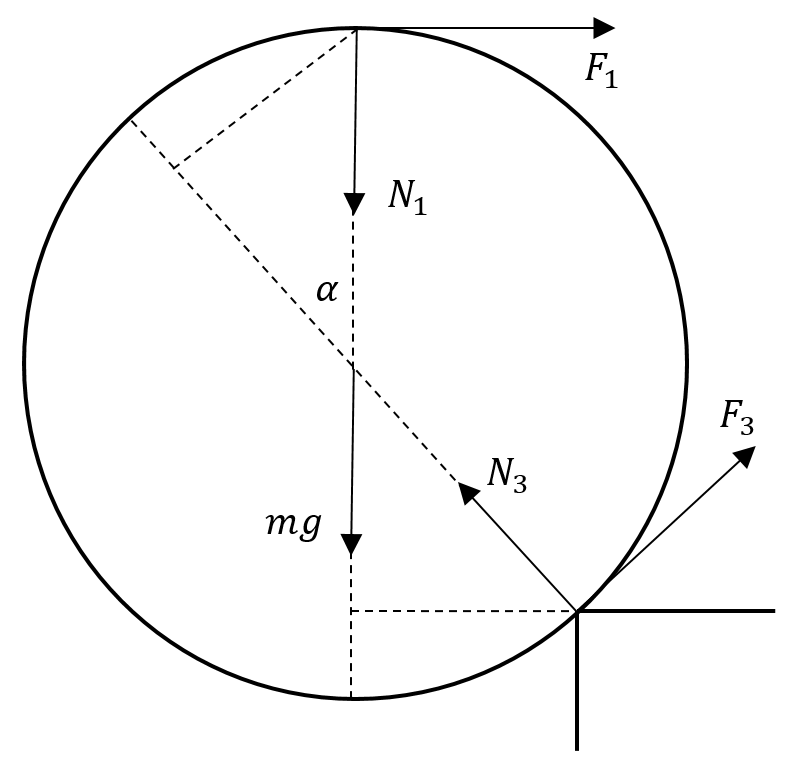
\includegraphics[width = \textwidth]{S-2}
        \caption{Forces on the cylinder.}
        \labelf{S-2}
    \end{subfigure}
    
    \caption{The forces in the system. $F_i$ are the friction forces.}
    \labelf{S-1-2}
    \vspace{-4cm}
\end{wrapfigure}

The forces acting on the cylinder and the plank are shown on \reff{S-1-2}

From the equilibrium (both translational and rotational) on the plank we get
\begin{equation}
\begin{split}
    N_1 &= N_2 = \frac{Mg}{2} \\
    F_1 &= F_2    
\end{split}
\end{equation}
and the equations for equilibrium on the cylinder,
particularly torques against the center,
torques against the cylinder's top point and
torques against the cylinder-table touching point are respectively
\begin{equation}
\begin{split}
    F_1 &= F_3 \\
    R N_3 \sin{\alpha} &= R F_3 (1 + \cos{\alpha}) \\
    R (mg + N_1) \sin{\alpha} &= R F_1 (1 + \cos{\alpha})
\end{split}
\end{equation}
where $R$ is the radius of the cylinder.
It is now easy to see, that
\begin{equation}
    F_1 = \frac{(2m + M) g \sin{\alpha}}{2 (1 + \cos{\alpha})}
\end{equation}

For the required values of friction coefficients we simply get
\begin{equation}
\begin{split}
    \mu_{c,t} &> \frac{F_3}{N_3} = \frac{\sin{\alpha}}{1 + \cos{\alpha}} \\
    \mu_{c,p / p,t} &> \frac{F_2}{N_2} = \frac{F_1}{N_1} = \frac{\sin{\alpha}}{1 + \cos{\alpha}} \inb({1 + \frac{2m}{M}})
\end{split}
\end{equation}
